\section{J1744$-$1134}
\label{sec:J1744}

\subsection{Epoch-wise DM(t) correction}
\begin{center}
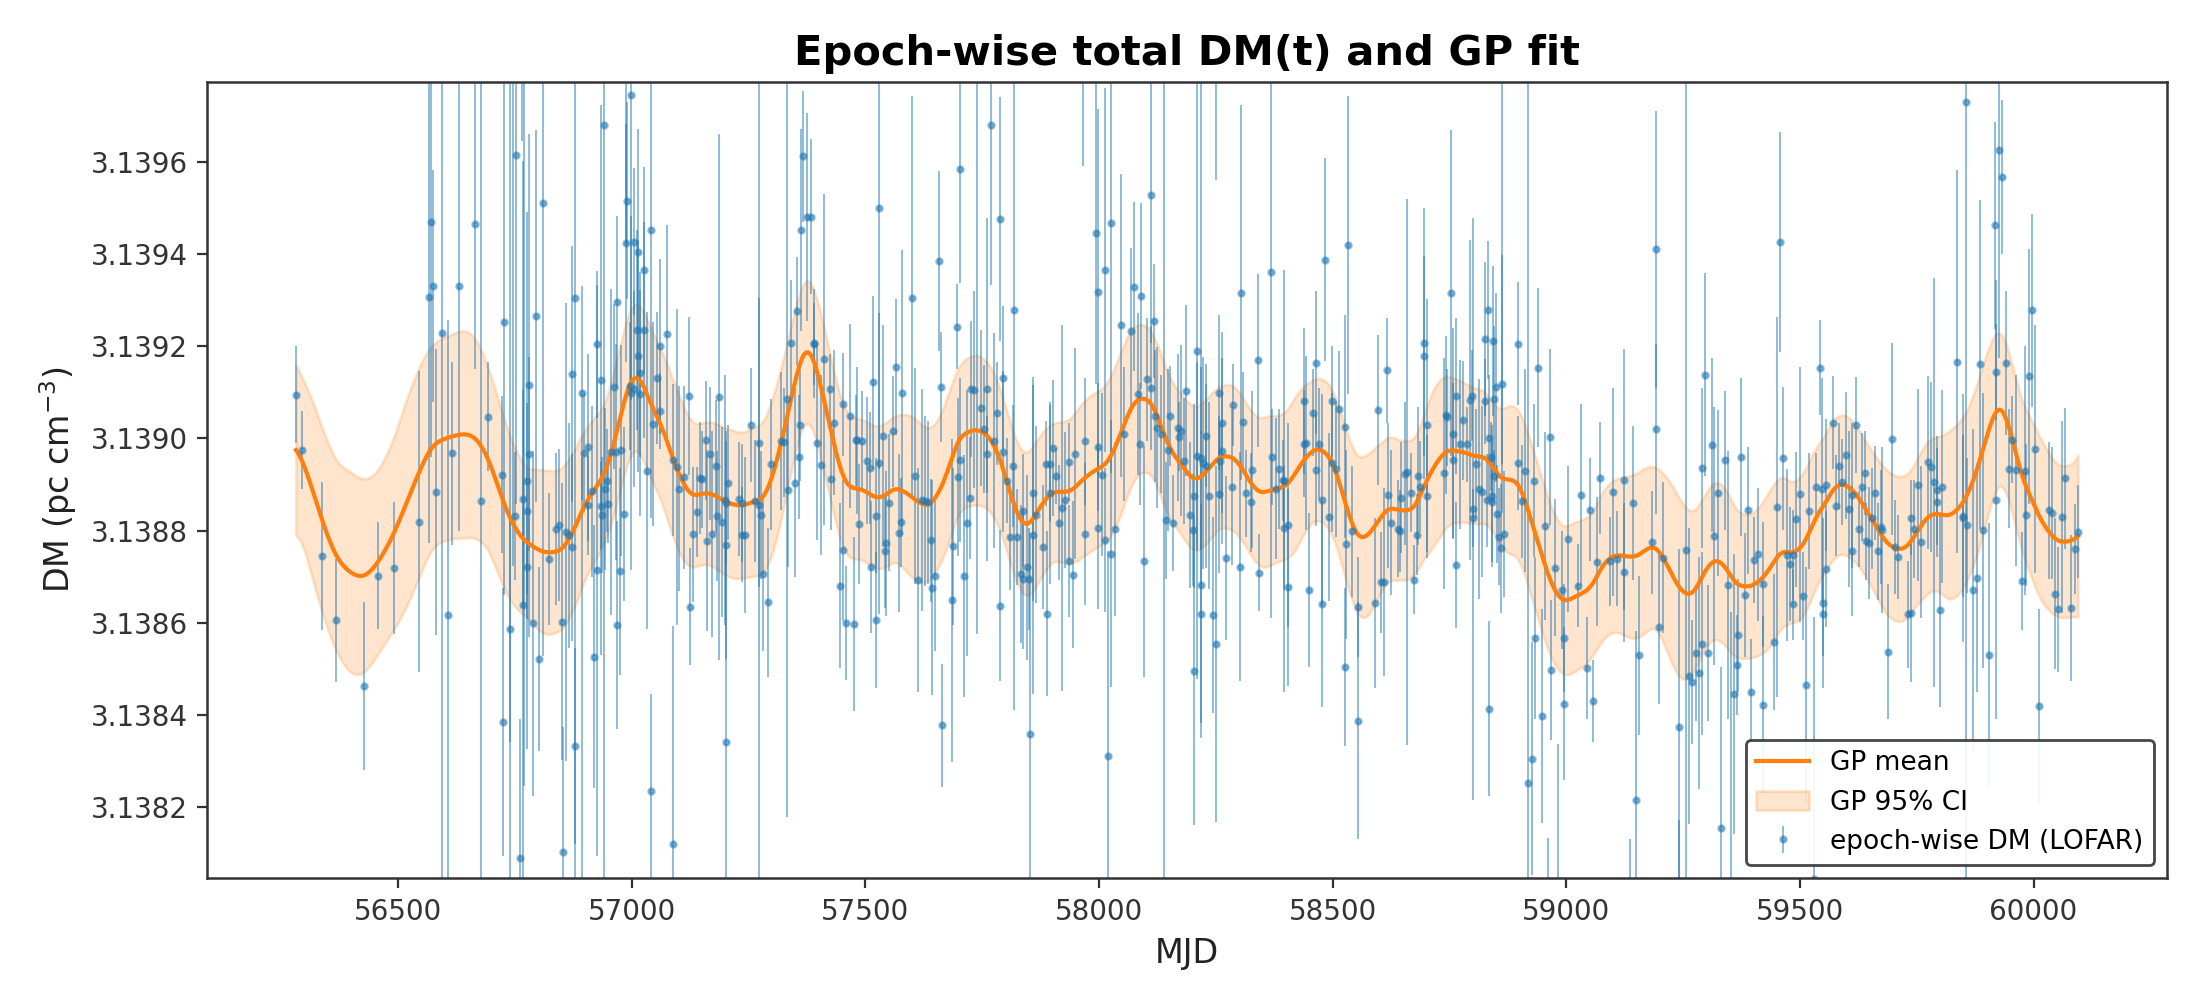
\includegraphics[width=0.8\textwidth]{../J1744-1134/dm_correction_out/dm_timeseries.png}
\end{center}

\subsection{Effect on residuals}
\begin{center}
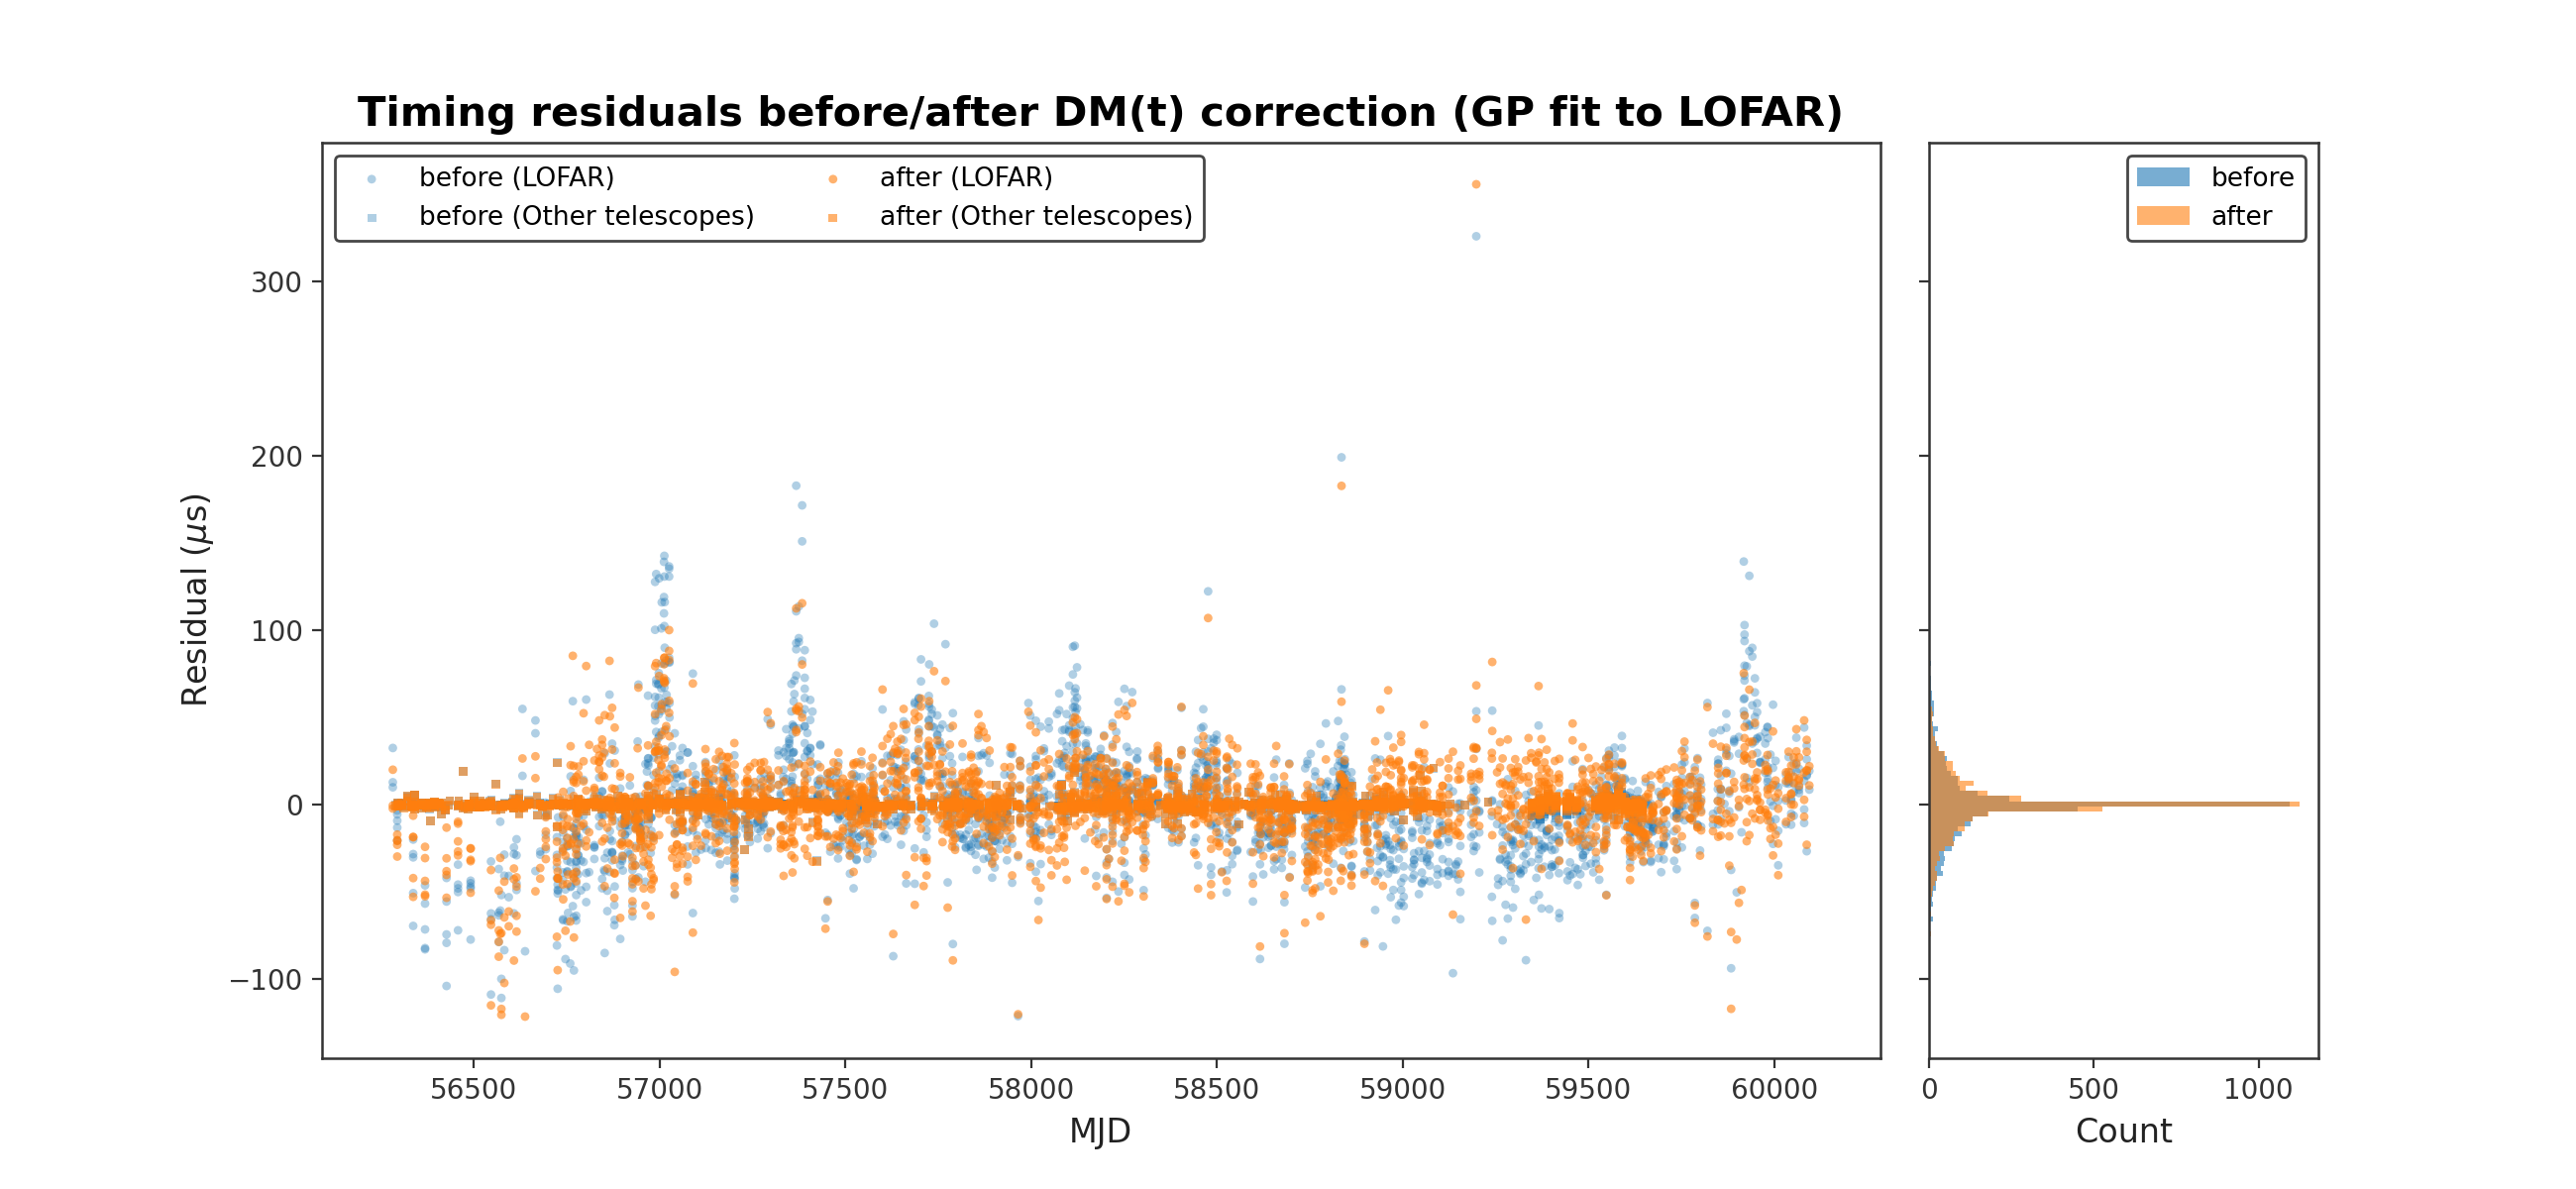
\includegraphics[width=0.8\textwidth]{../J1744-1134/dm_correction_out/residuals_pre_post.png}
\end{center}

\subsection{Noise-model comparisons}

\colorkeytable{J1744-1134}

\cmpjoint{../plot_output/compare/J1744-1134.pdf}{highfreq\_corrected: rnonly vs dmrn}
\cmpjoint{../plot_output/compare/J1744-1134_lofaronly_corrected_rnonly_vs_dmrn.pdf}{lofaronly\_corrected: rnonly vs dmrn}
\cmpjoint{../plot_output/compare/J1744-1134_corrected_dmrn_3way.pdf}{corrected, dmrn: highfreq vs lofaronly vs combined}
\cmpone{../plot_output/compare/J1744-1134_corrected_rnonly_3way.pdf}{corrected, rnonly: highfreq vs lofaronly vs combined}
\cmpjoint{../plot_output/compare/J1744-1134_uncorrected_vs_corrected.pdf}{combined: uncorrected vs corrected (dmrn)}
\cmpjoint{../plot_output/compare/J1744-1134_lofaronly_corr_vs_uncorr_dmrn.pdf}{lofaronly: corrected vs uncorrected (DM+RN)}
\cmpone{../plot_output/compare/J1744-1134_lofaronly_corr_vs_uncorr_rnonly.pdf}{lofaronly: corrected vs uncorrected (RN only)}
\cmpjoint{../plot_output/compare/J1744-1134_rnonly-corrected_vs_dmrn-uncorrected.pdf}{combined\_corrected:rnonly vs combined\_uncorrected:dmrn}
\cmpjoint{../plot_output/compare/J1744-1134_lofaronly_uncorrected_rnonly_vs_dmrn.pdf}{lofaronly\_uncorrected: rnonly vs dmrn}
\cmpone{../plot_output/compare/J1744-1134_rnonly_highfreqU_vs_lofaronlyU_vs_combinedU.pdf}{RN only, uncorrected: highfreq vs lofaronly vs combined}

\subsection{DM(t): GP reconstruction vs epoch-wise}
\cmpwide{../plot_output/compare/J1744-1134_dm_timeseries_ew_vs_gp.pdf}{combined\_corrected:dmrn DM GP vs the original epoch-wise curve}

\subsection{Interpretation}

J1744$-$1134 is the one pulsar where the correction behaves as intended: the
red-noise posterior overlaps substantially across all three tests ---
\emph{combined\_corrected:rnonly} vs \emph{combined\_uncorrected:dmrn},
and \emph{combined\_corrected:rnonly} vs \emph{highfreq\_corrected:rnonly}
--- with no strong dependence on whether LOFAR is included or whether DM is
modelled explicitly. The caveat: J1744$-$1134 is close to the ecliptic, so
part of what the epoch-wise correction measures and removes near solar
conjunction may be solar-wind signal rather than pure interstellar DM(t).
The clean agreement seen here is consistent with the correction working,
but is not on its own proof that it is working \emph{for the right reason}.

The three-way station split confirms this directly: under both
\emph{rnonly} and \emph{dmrn}, \emph{combined} tracks \emph{highfreq}
closely, even though \emph{lofaronly} alone finds a distinct peak in each
case --- a higher-amplitude red noise under \emph{rnonly}, and a DM GP
offset in amplitude (though not spectral index) from \emph{highfreq}'s own
under \emph{dmrn}. In other words, LOFAR's own slightly different
preference is simply outweighed once merged with the more numerous
high-frequency data here, rather than \emph{combined} inheriting it the way
it does for J1012+5307 and J1640+2224. Unlike those two pulsars, the
corrected-data DM GP does \emph{not} fully rail to zero amplitude when
isolated to \emph{lofaronly} alone; it retains a modest, well-localized
peak ($\gamma<1$, $\log_{10}A\approx-14$), distinct from but closer to the
uncorrected DM GP's own peak than in either other pulsar. This is
consistent with the ecliptic-proximity caveat already raised: some
residual, DM-like power survives the correction here, plausibly solar-wind
signal that NE\_SW$\to$0 alone does not remove. The three-way \emph{rnonly}
split among the three \emph{uncorrected} station sets still shows three
disjoint peaks ordered by frequency band, confirming that even in this
best-behaved case, an achromatic-only fit on uncorrected data is sensitive
to which stations are included --- the correction's job is still necessary
here, it is simply more complete than for the other two pulsars.
